\mode*
\part{Linux Programming Environment}
\lecture{programming environment}{env}

\section{C Programming Environment}
\label{sec:c-programming-basics}

\begin{frame}{Program Languages}
  \begin{block}{Machine code}
    The \alert{binary numbers} that the CPUs can understand.
    \begin{center}{\ttfamily
      100111000011101111001111 ... and so on ...}
    \end{center}
    People don't think in numbers.
  \end{block}
  \begin{block}{Assembly language --- friendly to humans}
    \begin{center}
      \mode<beamer>{ \includegraphics[width=.4\textwidth]{asm-sample-asm} }%
      \mode<article>{ \includegraphics[width=.2\textwidth]{asm-sample-asm} }
    \end{center}
    \begin{description}
    \item[Assemblers] translate the ASM programs to machine code
    \end{description}
  \end{block}
\end{frame}

\begin{frame}
  \begin{block}{High level languages}
    Even easier to understand by humans. Examples:
    \begin{itemize}
    \item C\tikzmark{clang}
    \item FORTRAN\tikzmark{fortran}
    \item Java\tikzmark{java}
    \item C++\tikzmark{cpp}
    \item ...\tikzmark{more}
    \end{itemize}\pause
    \begin{description}
    \item[Compilers] do the translation work
    \end{description}
  \end{block}
  \begin{tikzpicture}[remember picture,overlay,
    every node/.style={ellipse,red,opacity=.4,draw},
    every to/.style={append after command={[->,black!30,thick]}}
    ]
    \node (asm) at ($(pic cs:java) + (3,.5ex)$) {Assembly};
    \node (bin) [right=of asm] {Binary};
    \draw ($(pic cs:clang)+(0,.5ex)$) to [bend left=20] (asm);
    \draw ($(pic cs:fortran)+(0,.5ex)$) to [bend left=15] (asm);
    \draw ($(pic cs:java)+(0,.5ex)$) to (asm);
    \draw ($(pic cs:cpp)+(0,.5ex)$) to [bend right=15] (asm);
    \draw ($(pic cs:more)+(0,.5ex)$) to [bend right=20] (asm);
    \draw (asm) to (bin);
    \end{tikzpicture}
\end{frame}

\subsection{The Tool Chain}
\label{sec:tool-chain}

\begin{frame}{Compilation}
  \begin{center}
    \mode<beamer>{ \includegraphics[width=\textwidth]{tool-chain} }%
    \mode<article>{ 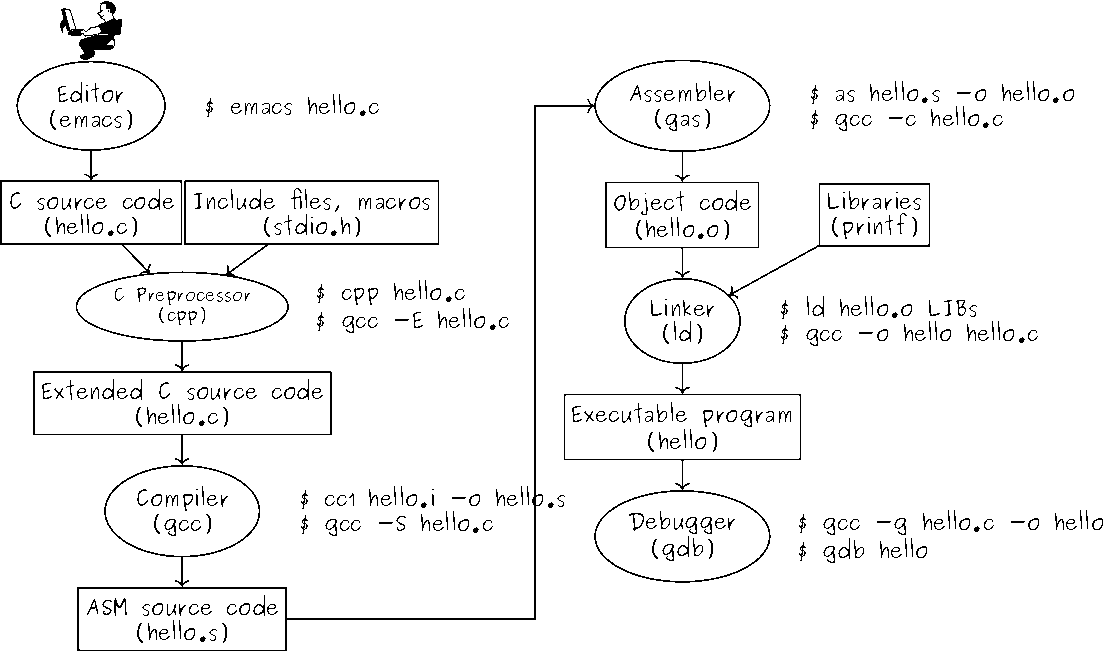
\includegraphics[width=.9\textwidth]{tool-chain-bw} }
  \end{center}
\end{frame}

\begin{description}
\item[Source code] written by programmer in high-level language, in our case in
  \texttt{C}. We write c source code with a \emph{text editor}, such as \texttt{emacs},
  \texttt{vim}, etc.
\item[Preprocessing] is the first pass of any C compilation. It processes
  \texttt{include-files}, \texttt{conditional compilation instructions} and
  \texttt{macros}.
  \begin{description}
  \item[cpp] The GNU C preprocessor
    \begin{itemize}
    \item[\$] \texttt{gcc -E hello.c}
    \end{itemize}
  \end{description}
\item[{Compilation}] is the second pass. It takes the output of the preprocessor, and the
  \texttt{source code}, and generates \texttt{assembly source code}.
  \begin{description}
  \item[gcc/g++] GNU C/C++ compiler
    \begin{itemize}
    \item[\$] \texttt{gcc -S hello.c}
    \end{itemize}
  \end{description}
\item[Assembly] is the third stage of compilation. It takes the assembly source code and
  produces an assembly listing with offsets. The assembler output is stored in an
  \texttt{object file}.
  \begin{description}
  \item[as] the portable GNU assembler
    \begin{itemize}
    \item[\$] \texttt{gcc -c hello.c}
    \end{itemize}
  \end{description}
\item[Linking] is the final stage of compilation. It combines object code with predefined
  routines from \texttt{libraries} and produces the \texttt{executable program}.
  \begin{description}
  \item[ld] The GNU linker
    \begin{itemize}
    \item[\$] \texttt{gcc hello.c -lm}
    \end{itemize}
  \end{description}
\item[{Wrapper}] The whole compilation process is usually not done `by hand', but using a
  \texttt{wrapper} program that combines the functions of preprocessor(cpp),
  compiler(gcc/g++), assembler(as) and linker(ld).
  \begin{itemize}
  \item[\$] \texttt{gcc -Wall hello.c -lm -o hello}
  \end{itemize}
\end{description}

\begin{frame}{Compiler vs. Interpreter}
  \begin{iblock}{\texttt{hello.c}}
    \begin{minipage}{.4\linewidth}
      \mode<beamer>{ 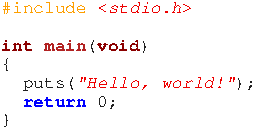
\includegraphics[width=\textwidth]{helloworld-c} }%
      \mode<article>{ \cfile{../src/helloworld.c} }
    \end{minipage}
    \begin{minipage}{.5\linewidth}
      \begin{itemize}
      \item[\$] \texttt{gcc -o hello hello.c}
      \item[\$] \texttt{./hello}
      \end{itemize}
    \end{minipage}
  \end{iblock}
  \begin{iblock}{\texttt{hello.sh}}
    \begin{minipage}{.4\linewidth}
      \mode<beamer>{ \includegraphics[width=\textwidth]{hello-sh} }%
      \mode<article>{ \shfile{../src/hello.sh} }
    \end{minipage}
    \begin{minipage}{.5\linewidth}
      \begin{enumerate}
      \item[\$] \texttt{chmod +x hello.sh}
      \item[\$] \texttt{./hello.sh}
      \end{enumerate}
    \end{minipage}
  \end{iblock}
  \begin{iblock}{\texttt{hello.py}}
    \begin{minipage}{.4\linewidth}
      \mode<beamer>{ 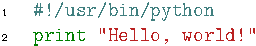
\includegraphics[width=\textwidth]{hello-py} }%
      \mode<article>{ \pyfile{../src/hello.py} }
    \end{minipage}
    \begin{minipage}{.5\linewidth}
      \begin{enumerate}
      \item[\$] \texttt{chmod +x hello.py}
      \item[\$] \texttt{./hello.py}
      \end{enumerate}
    \end{minipage}
  \end{iblock}
\end{frame}

\subsection{Header Files}
\label{sec:header-files}

\begin{frame}{Header Files}
  \begin{minipage}{.45\linewidth}
    \begin{iblock}{Why?}
      \mode<beamer>{ 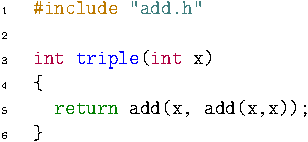
\includegraphics[width=\textwidth]{hdr1-c} }%
      \mode<article>{ \cfile{figs/hdr1.c} }
    \end{iblock}
  \end{minipage}\qquad
  \begin{minipage}{.45\linewidth}
    \begin{iblock}{Why not?}
      \mode<beamer>{ 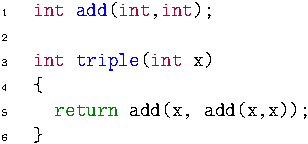
\includegraphics[width=\textwidth]{hdr2-c} }%
      \mode<article>{ \cfile{figs/hdr2.c} }
    \end{iblock}
  \end{minipage}\\[1ex]
  \begin{itemize}
  \item Ensure everyone use the same code
  \item Easy to share, upgrade, reuse
  \end{itemize}
  \begin{block}{In the header files\ldots}
    \begin{multicols}{2}
      \begin{itemize}
      \item function declarations
      \item macro definitions
      \item constants
      \item system wide global variables
      \end{itemize}
    \end{multicols}
  \end{block}
  \begin{itemize}
  \item[\$] \texttt{ls /usr/include/}
  \end{itemize}
\end{frame}

\subsubsection{A small software project}
\label{sec:small-softw-proj}

\begin{minipage}[t]{.45\linewidth}
\begin{block}{\texttt{Makefile}}
  \mkfile{../src/hdr/Makefile}
\end{block}  
\end{minipage}\qquad
\begin{minipage}[t]{.45\linewidth}
\begin{block}{\texttt{triple.c}}
  \cfile{../src/hdr/triple.c}
\end{block}  
\end{minipage}

\begin{minipage}[t]{.45\linewidth}
\begin{block}{\texttt{add.h}}
  \cfile{../src/hdr/add.h}
\end{block}
\end{minipage}\quad
\begin{minipage}[t]{.45\linewidth}
\begin{block}{\texttt{add3.c}}
  \cfile{../src/hdr/add3.c}
\end{block}  
\end{minipage}

\begin{description}
\item[\texttt{triple.c}] --- the main source file.
\item[\texttt{add.h}] --- macros and function prototypes. Like \texttt{stdio.h}, can be
  used by anyone.
\item[\texttt{add3.c}] --- function implementations. It's like a black box. Any changes
  made inside a block box are transparent to the calling functions.
\item[\texttt{Makefile}] --- managing the project.
\end{description}

\subsection{Library Files}
\label{sec:library-files}

\begin{frame}{Library Files}
  \begin{description}
  \item[A library] is a collection of pre-compiled object files which can be linked into programs.
  \item[Static libraries] \alert{\texttt{.a}} files. Very old ones, but still alive.
    \begin{itemize}
    \item[\$] \texttt{find /usr/lib -name "*.a"}
    \end{itemize}
  \item[Shared libraries] \alert{\texttt{.so}} files. The preferred ones.
    \begin{itemize}
    \item[\$] \texttt{find /usr/lib -name "*.so.*"}
    \end{itemize}
  \end{description}
\end{frame}

\begin{frame}{Example}
  \begin{iblock}{\texttt{calc.c}}
    \mode<beamer>{ 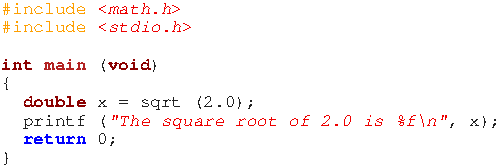
\includegraphics[width=\textwidth]{calc-c} }%
    \mode<article>{ \cfile{../src/calc.c} }
  \end{iblock}\ttfamily
  \begin{itemize}
  \item[\$] gcc -o calc calc.c \$(find /usr/lib -name libm.a) \correct
  \item[\$] gcc -o calc calc.c -lm \correct
  \item[\$] gcc -o calc -lm calc.c \Bad
  \end{itemize}
\end{frame}

\begin{itemize}
\item \url{https://www.linuxtopia.org/online_books/an_introduction_to_gcc/gccintro_18.html}
\end{itemize}

\begin{frame}
  \begin{block}{Static Linking}
    \begin{itemize}
    \item The entire program and all data of a process must be in physical memory for the
      process to execute
    \item The size of a process is thus limited to the size of physical memory
    \end{itemize}
  \end{block}
    \begin{center}
    \mode<beamer>{ 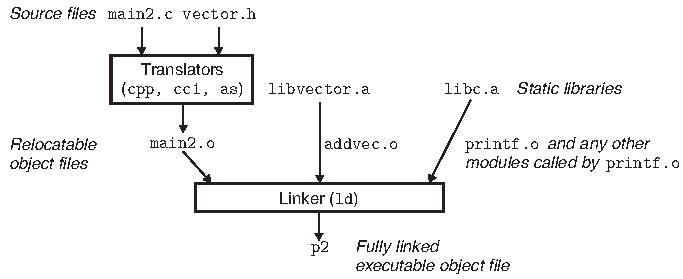
\includegraphics[width=\textwidth]{static-linking} }%
    \mode<article>{ 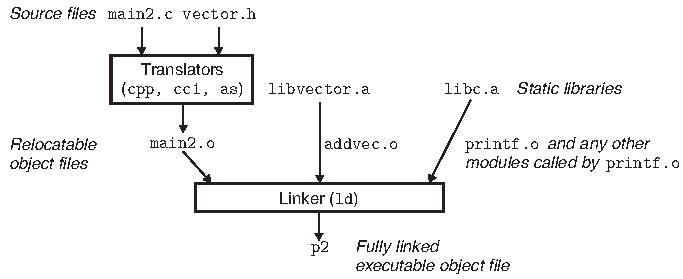
\includegraphics[width=.7\textwidth]{static-linking} }
  \end{center}
\end{frame}

\begin{frame}
  \begin{block}{Dynamic Linking}
    \begin{itemize}
    \item Only one copy in memory
    \item Don't have to re-link after a library update
    \end{itemize}
  \end{block}
  \begin{center}
    \mode<beamer>{ 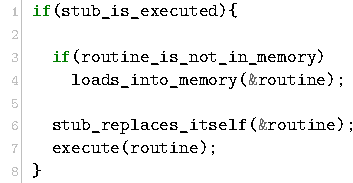
\includegraphics[width=.7\textwidth]{dynamic-linking} }%
    \mode<article>{ 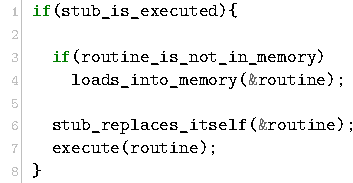
\includegraphics[width=.5\textwidth]{dynamic-linking} }
  \end{center}
\end{frame}

\begin{frame}{Build A Static Library}{Source codes}
  \begin{minipage}[t]{.47\linewidth}
    \begin{iblock}{\texttt{main.c}}
      \begin{center}
        \mode<beamer>{ \includegraphics[width=\textwidth]{main-c} }%
        \mode<article>{\cfile{../src/static/main.c}}
      \end{center}
    \end{iblock}
    \begin{iblock}{\texttt{lib.h}}
      \mode<beamer>{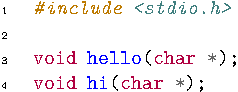
\includegraphics[width=.5\textwidth]{lib-h}}%
      \mode<article>{\cfile{../src/static/lib.h}}
    \end{iblock}
  \end{minipage}\qquad
  \begin{minipage}[t]{.43\linewidth}
    \begin{iblock}{\texttt{hello.c}}
      \begin{center}
        \mode<beamer>{ \includegraphics[width=\textwidth]{hello-c} }%
        \mode<article>{\cfile{../src/static/hello.c}}
      \end{center}
    \end{iblock}
    \begin{iblock}{\texttt{hi.c}}
      \begin{center}
        \mode<beamer>{ 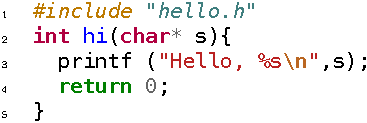
\includegraphics[width=\textwidth]{hi-c} }%
        \mode<article>{\cfile{../src/static/hi.c}}
      \end{center}
    \end{iblock}
  \end{minipage}
\end{frame}

\begin{frame}{Build A Static Library}{Step by step}
  \begin{enumerate}
  \item Get \alert{\texttt{hello.o}} and \alert{\texttt{hi.o}}
    \begin{itemize}
    \item[\$] \texttt{gcc -c hello.c hi.c}
    \end{itemize}
  \item Put \alert{\texttt{*.o}} into \alert{\texttt{libhi.a}}
    \begin{itemize}
    \item[\$] \texttt{ar crv libhi.a hello.o hi.o}
    \end{itemize}
  \item Use \alert{\texttt{libhi.a}}
    \begin{itemize}
    \item[\$] \texttt{gcc main.c libhi.a}
    \end{itemize}
  \end{enumerate}
\end{frame}

\begin{frame}{Build A Static Library}{Makefile}
  \begin{center}
    \mode<beamer>{ \includegraphics[width=.8\textwidth]{makefile-a} }%
    \mode<article>{\mkfile{../src/static/Makefile}}
  \end{center}
\end{frame}

\begin{frame}{Build A Shared Library}{Source codes}
  \begin{iblock}{\texttt{hello.c}}
    \begin{center}
      \mode<beamer>{ \includegraphics[width=.8\textwidth]{hello-c-so} }%
      \mode<article>{\cfile{../src/shared/hello.c}}
    \end{center}
  \end{iblock}
  \begin{minipage}{.35\linewidth}
    \begin{iblock}{\texttt{hello.h}}
      \mode<beamer>{ \includegraphics[width=\textwidth]{hello-h-so} }%
      \mode<article>{\cfile{../src/shared/hello.h}}
    \end{iblock}
  \end{minipage}\qquad
  \begin{minipage}{.36\linewidth}
    \begin{iblock}{\texttt{hi.c}}
      \mode<beamer>{ \includegraphics[width=\textwidth]{hi-c-so} }%
      \mode<article>{\cfile{../src/shared/hi.c}}
    \end{iblock}
  \end{minipage}
\end{frame}

\begin{frame}{Build A Shared Library}{Step by step}
  \begin{enumerate}
  \item Get \alert{\texttt{hi.o}}
    \begin{itemize}
    \item[\$] \texttt{gcc -fPIC -c hi.c}
    \end{itemize}
  \item Get \alert{\texttt{libhi.so}}
    \begin{itemize}
    \item[\$] \texttt{gcc -shared -o libhi.so hi.o}
    \end{itemize}
  \item Use \alert{\texttt{libhi.so}}
    \begin{itemize}
    \item[\$] \texttt{gcc -L. -Wl,-rpath=. hello.c -lhi}
    \end{itemize}
  \item Check it
    \begin{itemize}
    \item[\$] \texttt{ldd a.out}
    \end{itemize}
  \end{enumerate}
\end{frame}

\begin{frame}{Build A Shared Library}{Makefile}
  \begin{center}
    \mode<beamer>{ \includegraphics[width=\textwidth]{makefile-so} }%
    \mode<article>{\mkfile{../src/shared/Makefile}}
  \end{center}
\end{frame}

\begin{description}
\item[Position Independent Code (PIC)] Unlike executables, when shared libraries are being
  built, the linker can't assume a known load address for their code. When translated to
  x86 assembly, this will involve lots of \texttt{mov} instruction to pull the value of
  some variable from its location in memory into a register. \texttt{mov} requires an
  absolute address - so how does the linker know which address to place in it? The answer
  is - it doesn't. As I mentioned above, shared libraries have no pre-defined load address
  - it will be decided at runtime.

  In Linux, the dynamic loader is a piece of code responsible for preparing programs for
  running. One of its tasks is to load shared libraries from disk into memory, when the
  running executable requests them. When a shared library is loaded into memory, it is
  then adjusted for its newly determined load location. It is the job of the dynamic
  loader to solve the problem presented in the previous paragraph.

  The idea behind PIC is simple - add an additional level of indirection to all global
  data and function references in the code. By cleverly utilizing some artifacts of the
  linking and loading processes, it's possible to make the text section of the shared
  library truly \emph{position independent}, in the sense that it can be easily mapped
  into different memory addresses without needing to change one bit.
  \begin{itemize}
  \item
    \url{https://eli.thegreenplace.net/2011/08/25/load-time-relocation-of-shared-libraries/}
  \item
    \url{https://eli.thegreenplace.net/2011/11/03/position-independent-code-pic-in-shared-libraries/}
  \item \url{https://en.wikipedia.org/wiki/Position-independent_code}
  \item \url{https://en.wikipedia.org/wiki/Relocation_(computing)#Load-time}
  \item
    \url{https://stackoverflow.com/questions/813980/why-isnt-all-code-compiled-position-independent}
  \item \url{https://eklitzke.org/position-independent-executables}
  \item
    \url{http://davidad.github.io/blog/2014/02/19/relocatable-vs-position-independent-code-or/}
  \item
    \url{https://www.codeproject.com/Articles/1032231/What-is-the-Symbol-Table-and-What-is-the-Global-Of}
  \item \url{https://www.technovelty.org/linux/plt-and-got-the-key-to-code-sharing-and-dynamic-libraries.html}
  \end{itemize}
\end{description}

\begin{frame}{GNU C Library}
  \begin{minipage}{.55\linewidth}
    Linux API > POSIX API
    \ttfamily
    \begin{itemize}
    \item[\$] man 7 libc
    \item[\$] man 3 intro
    \item[\$] man gcc
    \item[\$] info gcc
    \item[\debian] sudo apt install gcc-doc
    \end{itemize}
  \end{minipage}
  \begin{minipage}{.4\linewidth}
    \begin{center}
      \mode<beamer>{ 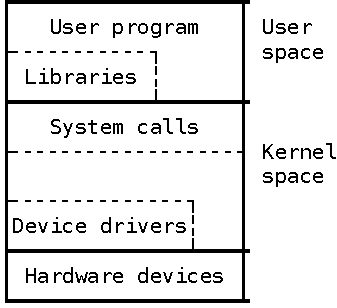
\includegraphics[width=\textwidth]{api} }%
      \mode<article>{ 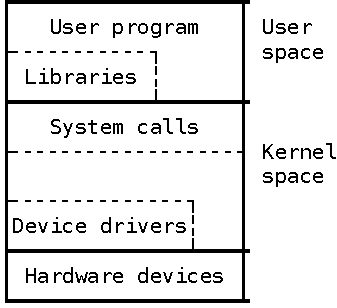
\includegraphics[width=.5\textwidth]{api} }
    \end{center}
  \end{minipage}
\end{frame}

\subsection{Error Handling}
\label{sec:error-handling}

\begin{frame}{\texttt{errno.h}}
  \begin{center}
    \mode<beamer>{ 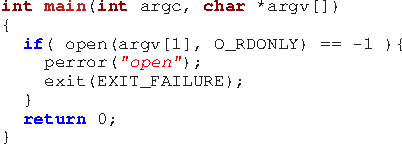
\includegraphics[width=.6\textwidth]{perror-c} }%
    \mode<article>{\cfile{../src/perror.c}}
  \end{center}\ttfamily
  \begin{itemize}
  \item[\$] man errno
  \item[\$] man errno.h
  \item[\$] man perror
  \end{itemize}
\end{frame}

\begin{itemize}
\item \citetitle[Sec.~1.7]{stevens2013advanced}
\item \url{https://stackoverflow.com/questions/30078281/raise-error-in-a-bash-script}
\end{itemize}

\subsection{The Make Utility}

\begin{frame}{The Make Utility}
  To compile a single C program:
  \begin{itemize}
  \item[\$] \cmd{gcc hello.c -o hello}\quad{\Huge \correct}\textsubscript{{\tiny OK. But\ldots}}
    % \tikz \node [opacity=.4,red,scale=3,inner
    % sep=0pt,label={[below=2.5ex,right]{\tiny OK. But...}}] {\Checked};
  \end{itemize}
  \begin{iblock}{What if you have a large project with 1000+ files?}
    \begin{center}
      \mode<beamer>{ 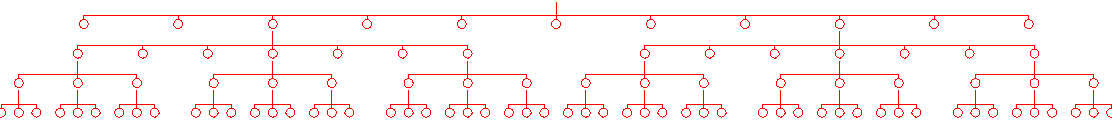
\includegraphics[width=\textwidth]{tree} }%
      \mode<article>{ 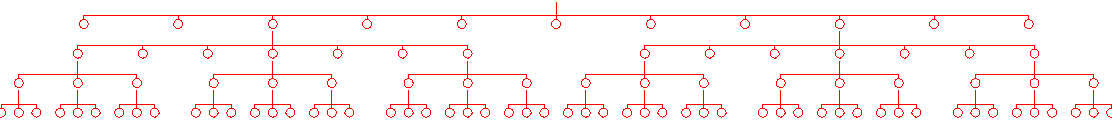
\includegraphics[width=.5\textwidth]{tree} }
    \end{center}
    \begin{description}
    \item[Linux 4.9 source tree:] 3799 directories, 55877 files
    \end{description}
  \end{iblock}
  \begin{description}
  \item[make:] help you maintain your programs.
  \end{description}
\end{frame}

\begin{frame}{Makefile}
  \begin{iblock}{}
      \mode<beamer>{ 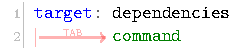
\includegraphics[width=.5\textwidth]{mktab1} }%
      \mode<article>{ 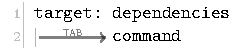
\includegraphics[width=.3\textwidth]{mktab1-bw} }
  \end{iblock}
  \begin{iblock}{Example}
      \mode<beamer>{ 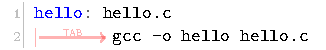
\includegraphics[width=.6\textwidth]{mktab2} }%
      \mode<article>{ 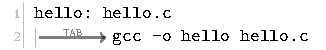
\includegraphics[width=.4\textwidth]{mktab2-bw} }
  \end{iblock}
  \begin{itemize}
  \item[\$] \cmd{info make makefiles}
  \end{itemize}
\end{frame}

\begin{frame}{Makefile}
  \begin{minipage}{.75\linewidth}
    \mode<beamer>{ 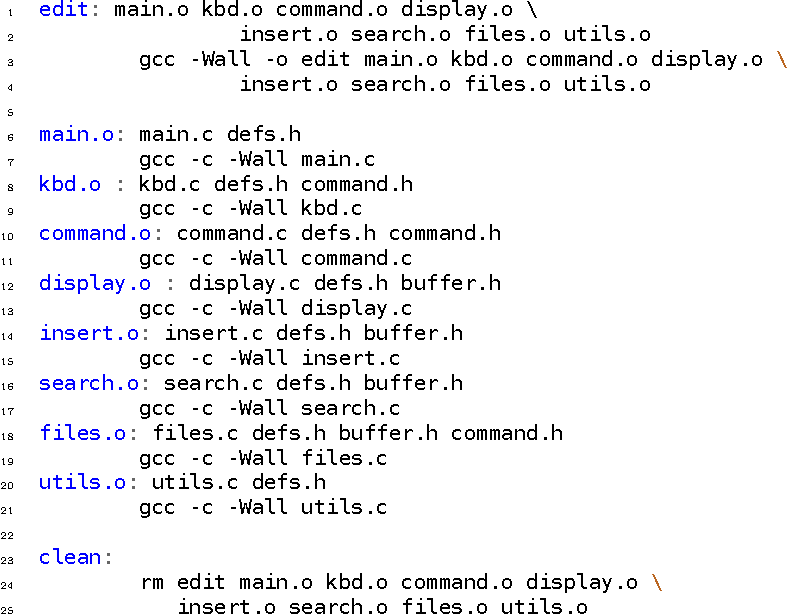
\includegraphics[width=1.1\textwidth]{Makefile2-mk} }%
    \mode<article>{\mkfile{figs/Makefile2}}
  \end{minipage}
  \begin{minipage}{.2\linewidth}
    \begin{center}
      \mode<beamer>{ 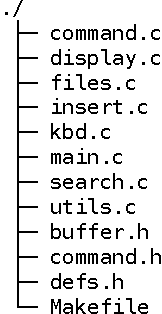
\includegraphics[width=\textwidth]{make-dir-tree} }%
      \mode<article>{ 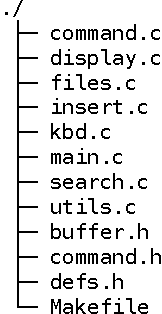
\includegraphics[width=.7\textwidth]{make-dir-tree} }
    \end{center}
  \end{minipage}
\end{frame}

\subsection{Version Control}
\label{sec:version-control}

\begin{frame}{git}
  \begin{block}{To create a new local git repo}
    In your source code directory, do:\ttfamily
    \begin{itemize}
    \item[\$] git init
    \item[\$] git add .
    \item[\$] git commit -m "something to say\ldots"
    \end{itemize}
  \end{block}
  \begin{block}{To clone a remote repo}
    Example:\ttfamily
    \begin{itemize}
    \item[\$] git clone https://github.com/wx672/lecture-notes.git
    \item[\$] git clone https://github.com/wx672/dotfile.git
    \end{itemize}
  \end{block}
\end{frame}

\begin{frame}
  \begin{block}{Most commonly used git Commands}\ttfamily
    \begin{itemize}
    \item[\$] git add filename[s]
    \item[\$] git rm filename[s]
    \item[\$] git commit
    \item[\$] git status\qquad\CMD{git log}\qquad\CMD{git diff}
    \item[\$] git push\qquad\CMD{git pull}
    \item[\$] git help \{add,rm,commit,\ldots\}
    \end{itemize}
  \end{block}
  \begin{multicols}{2}
    \begin{itemize}
    \item[\$] man gittutorial
    \item[\$] man gittutorial-2
    \item[\debian] sudo apt install git
    \item[\github] \url{https://github.com}
    \end{itemize}
  \end{multicols}
\end{frame}

\subsection{Manual Pages}
\label{sec:manual-pages}

\begin{frame}{Man page}{Layout}
  \begin{center}
    \mode<beamer>{ 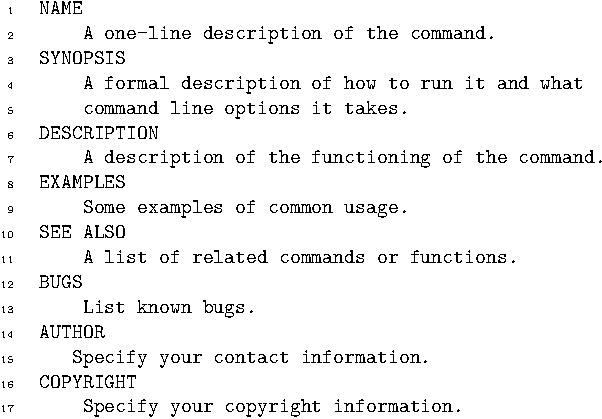
\includegraphics[width=.8\textwidth]{manpage-txt} }%
    \mode<article>{ 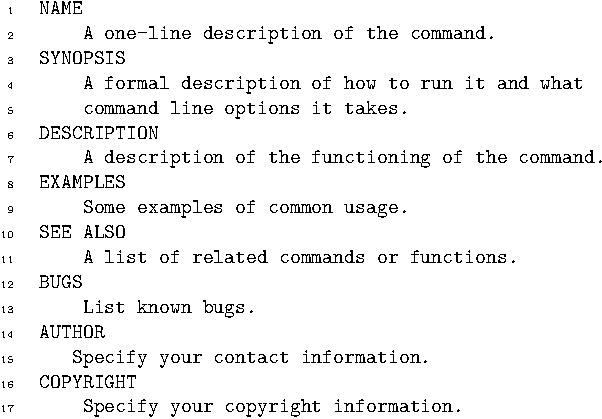
\includegraphics[width=.5\textwidth]{manpage-txt} }
  \end{center}
\end{frame}

\begin{frame}{Man Page}{Groff source code}
  \begin{minipage}[b]{.6\linewidth}
    \begin{center}
      \mode<beamer>{ 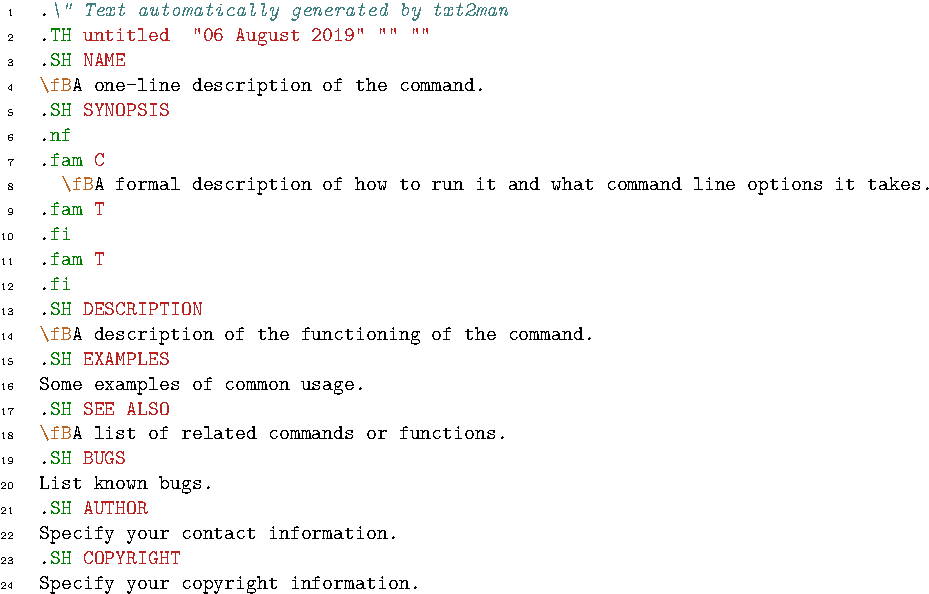
\includegraphics[width=1.6\textwidth]{manpage-1} }%
      \mode<article>{ 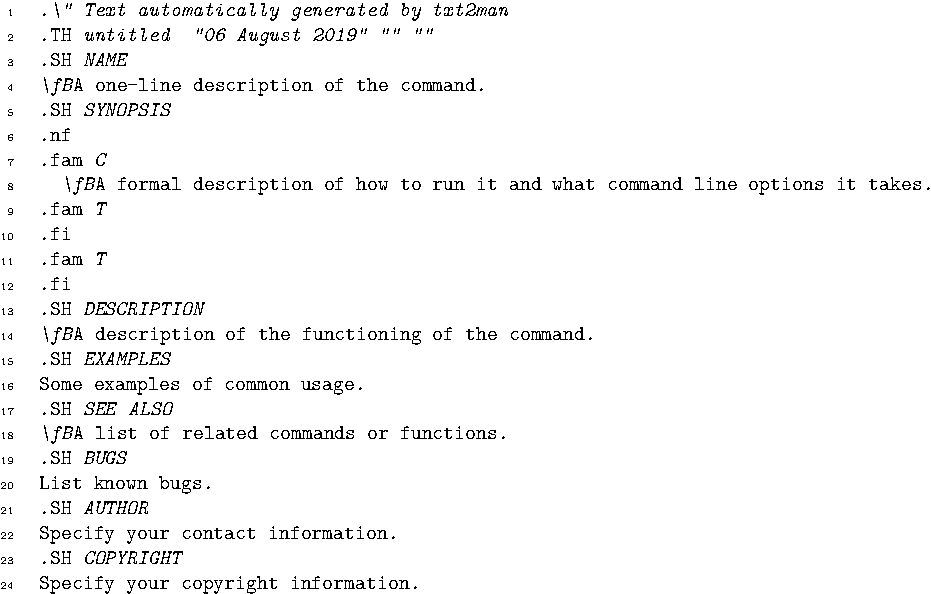
\includegraphics[width=1.2\textwidth]{manpage-1-bw} }
    \end{center}
  \end{minipage}
  \begin{minipage}[b]{.35\linewidth}\ttfamily
    \begin{itemize}
    \item[\$] man 7 groff
    \item[\$] man txt2man
    \item[\$] man a2x
    \item[\$] ls /usr/share/man
    \end{itemize}
  \end{minipage}
\end{frame}

\subsection{A Sample GNU Package}
\label{sec:sample-gnu-package}

\begin{frame}{How to ``Do one thing, and do it well''?}  
  \begin{itemize}
  \item[\$] \cmd{apt source hello}
  \end{itemize}
\end{frame}

\subsection{Pointers in C}
\label{sec:pointers-c}

\begin{frame}{Pointers}
  \begin{center}
    \mode<beamer>{ \includegraphics[width=.9\textwidth]{ptr1-code-c} }%
    \mode<article>{\cfile{../src/ptr1-code.c}}
  \end{center}
  \begin{center}
    \mode<beamer>{ \includegraphics[width=\textwidth]{ptr1} }%
    \mode<article>{ \includegraphics[width=.6\textwidth]{ptr1} }
  \end{center}
\end{frame}

\begin{frame}{Pointer Operators}
  \begin{itemize}
  \item[\&] returns the \alert{address} of a thing
  \item[{\dejavu ✶}] return the \alert{object (thing)} to which a pointer points at
  \end{itemize}
  \begin{block}{\texttt{int thing; int *thing\_ptr;}}
    \begin{center}
      \begin{tabular}{>{\ttfamily}rl}\hline
        \thead{C Code} & \thead{Description}            \\\hline
        thing          & the variable named `thing'     \\
        \&thing        & address of `thing' (a pointer) \\
        *thing         & \wrong{} \texttt{thing} is not a pointer\\
        thing\_ptr     & pointer to an int              \\
        *thing\_ptr    & the int variable at the address \texttt{thing\_ptr} points
                      to                                \\
        \&thing\_ptr   & odd, a pointer to a pointer    \\\hline
      \end{tabular}
    \end{center}
  \end{block}
\end{frame}

\begin{frame}
  \begin{iblock}{Example}
    \begin{center}
      \mode<beamer>{ \includegraphics[width=.9\textwidth]{ptr2-code-c} }%
      \mode<article>{\cfile{../src/ptr2-code.c}}
    \end{center}
  \end{iblock}
  \begin{center}
    \mode<beamer>{ \includegraphics[width=.8\textwidth]{ptr2} }%
    \mode<article>{ \includegraphics[width=.4\textwidth]{ptr2} }
  \end{center}
\end{frame}

\begin{frame}
  \begin{iblock}{Invalid operation}
    \begin{center}
      \mode<beamer>{ 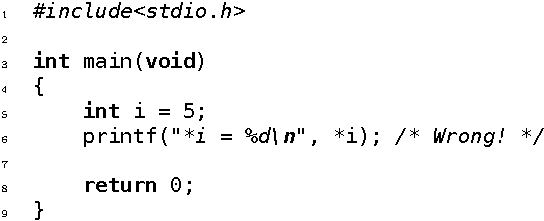
\includegraphics[width=.7\textwidth]{ptr2-wrong1-c} }%
      \mode<article>{\cfile{../src/ptr2-wrong1.c}}
    \end{center}
    \mode<article>{
      In the \texttt{printf()} statement, it's trying to treat \texttt{i} as a pointer.
    }
  \end{iblock}
  \begin{iblock}{Invalid memory access}
    \begin{center}
      \mode<beamer>{ 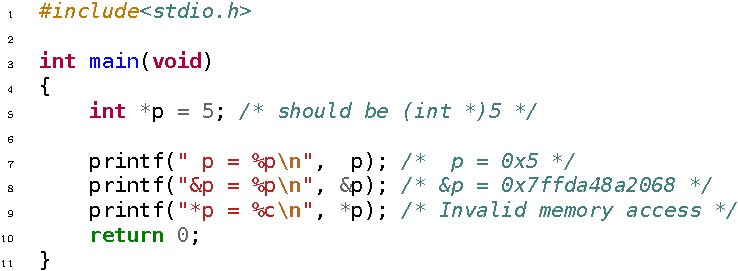
\includegraphics[width=\textwidth]{ptr2-wrong2-c} }%
      \mode<article>{ \cfile{../src/ptr2-wrong2.c} }
    \end{center}
    \mode<article>{This is trying to treat the value of \texttt{p} as a memory
      address. But the memory address \texttt{5} is not accessible by this program.}
  \end{iblock}
\end{frame}

\begin{frame}{Call By Value}
  \begin{center}
    \mode<beamer>{
      \includegraphics[width=.8\textwidth]{ptr4-wrong-c}\tikzmark{ptr4wrong}
      \pause
      \begin{tikzpicture}[remember picture,overlay]
        \node at ($(pic cs:ptr4wrong)+(0,2)$) [opacity=.4,scale=7] {\wrong};
      \end{tikzpicture}}%    
    \mode<article>{\cfile{../src/ptr4-wrong.c}}
  \end{center}
  \begin{description}
  \item[Call by value:] only the \alert{value} of `\texttt{count}' is handed to the
    function \texttt{inc\_count()}
  \end{description}
\end{frame}

\begin{frame}
  \begin{iblock}{Solution 1: return}
    \begin{center}
      \mode<beamer>{ \includegraphics[width=.7\textwidth]{ptr4-ok-c}%
        \begin{tikzpicture}[remember picture,overlay]
          \node at ($(pic cs:ptr4ok)+(0,2)$) [opacity=.4,scale=10] {\correct};
        \end{tikzpicture}}%
    \end{center}
    \mode<article>{\cfile{../src/ptr4-ok.c}%
      \begin{enumerate}
      \item read the \emph{value} of \texttt{count}, and pass it to \texttt{inc\_count()};
      \item \texttt{inc\_count()} uses the \emph{value} of \texttt{count} to do the
        calculations;
      \item return the result to \texttt{main()}.
      \end{enumerate}}
  \end{iblock}
\end{frame}

\begin{frame}%{Pointers as Function Arguments}
  \begin{iblock}{Solution 2: Call by reference}
    \begin{center}
      \mode<beamer>{ \includegraphics[width=.6\textwidth]{ptr4-c}%
        \begin{tikzpicture}[remember picture,overlay]
          \node at ($(pic cs:ptr4)+(0,2)$) [opacity=.4,scale=10] {\correct};
        \end{tikzpicture}}%
    \end{center}
    \mode<article>{\cfile{../src/ptr4.c}%
      \begin{enumerate}
      \item pass the address of \texttt{count} to \texttt{inc\_count()};
      \item \texttt{inc\_count()} operates directly on \texttt{count}.
      \end{enumerate}}
  \end{iblock}
  \begin{description}
  \item[More efficient than solution 1] Imagining you are operating on a large data
    structure rather than an \texttt{int}
  \end{description}
\end{frame}

\subsection{Pointers and Arrays}

\begin{frame}
  \begin{minipage}[t]{.45\linewidth}
    \includegraphics[width=\textwidth]{array2-c}
  \end{minipage}\quad
  \begin{minipage}[t]{.5\linewidth}
    \includegraphics[width=\textwidth]{array2-2-c}\tikzmark{array2-2}
    \mode<beamer>{
      \begin{tikzpicture}[remember picture,overlay]
        \node at ($(pic cs:array2-2)+(-.68,.95)$) [ellipse,opacity=.4,red,draw,thick,minimum
        width=1cm] {};
      \end{tikzpicture}}
    \mode<article>{
      \begin{tikzpicture}[remember picture,overlay]
        \node at ($(pic cs:array2-2)+(-.9,1.4)$) [ellipse,opacity=.4,red,draw,thick,minimum
        width=1.5cm] {};
      \end{tikzpicture}
      C automatically scales pointer arithmetic so that it works correctly, by
      incrementing/decrementing by the correct number of bytes. For example, in above
      program, the value of \texttt{pa} (\texttt{\&a[2]}) is \texttt{1008}, and the value
      of \texttt{a} (\texttt{\&a[0]}) is \texttt{1000}. But the result of ``\texttt{pa -
        a}'' is \texttt{2} rather than \texttt{8}. This means \texttt{pa} is \emph{two
        ints} ahead of \texttt{a}.}
  \end{minipage}
  \begin{center}
    \mode<beamer>{ \includegraphics[width=\textwidth]{array2-3} }%
    \mode<article>{ \includegraphics[width=.6\textwidth]{array2-3} }
  \end{center}
\end{frame}

\begin{frame}{Passing Arrays to Functions}
  \begin{block}{}
    When passing an array to a function, C will automatically change the array into a
    pointer.
  \end{block}
  \begin{center}
    \begin{minipage}{.53\linewidth}
      \mode<beamer>{ \includegraphics[width=\textwidth]{array3-1-c} }%
    \end{minipage}\quad
    \begin{minipage}{.4\linewidth}
      \mode<beamer>{ \includegraphics[width=\textwidth]{array3-2-c} }%
    \end{minipage}
  \end{center}
  \mode<article>{ \cfile{../src/array3.c} }
\end{frame}

\begin{frame}{Strings --- Arrays Of Characters}
  \begin{description}
  \item[Strings] are \alert{character arrays} with the additional special character
    ``\texttt{\textbackslash0}'' (\texttt{NUL}) at the end, e.g.:
    \ttfamily
    \begin{itemize}
    \item[] char system[] = "Linux";
    \item[] \begin{tabular}{*{6}{|c}|} \hline
              L&i&n&u&x&\textbackslash0\\\hline
            \end{tabular}
          \end{itemize}
  \end{description}
  \begin{iblock}{The most common string functions}
    \mode<beamer>{ \includegraphics[width=\textwidth]{string-funcs-c} }%
    \mode<article>{ \cfile{../src/string-funcs.c}}
  \end{iblock}
\end{frame}

\begin{frame}{Arrays Of Pointers}
  \begin{center}
    \mode<beamer>{ \includegraphics[width=.7\textwidth]{array4-c} }%
  \end{center}
  \mode<article>{ \cfile{../src/array4.c} }
\end{frame}

\begin{description}
\item[Once you've declared an array, you can't reassign it. Why?] Consider an assignment like

\begin{ccode}
char *my_str = "foo"; // Declare and initialize a char pointer.
my_str = "bar"; // Change its value.
\end{ccode}

The first line declares a char pointer and ``aims'' it at the first letter in \texttt{foo}. Since \texttt{foo} is a string constant, it resides somewhere in memory with all the other constants. When you reassign the pointer, you're assigning a new value to it: the address of \texttt{bar}. But the original string, \texttt{foo}, remains unchanged. You've moved the pointer, but haven't altered the data.

\emph{When you declare an array, however, you aren't declaring a pointer at all. You're reserving a certain amount of memory and giving it a name}. So the line

\begin{ccode}
char c[5] = "data";
\end{ccode}

starts with the string constant \texttt{data}, then allocates 5 new bytes, calls them \texttt{c}, and copies the string into them. You can access the elements of the array exactly as if you'd declared a pointer to them; arrays and pointers are (for most purposes) interchangeable in that way.

\emph{But since arrays are not pointers, you cannot reassign them}. You can't make
\texttt{c} ``point'' anywhere else, because it's not a pointer; it's the name of an area of
memory. For example,

\begin{ccode}
char c[5] = "data";
char b[5] = "beta";
b = c; /* Wrong! 'b[]' cannot be reassigned (pointing to elsewhere). */
\end{ccode}
\end{description}

\begin{itemize}
\item \url{https://stackoverflow.com/questions/17077505/string-pointer-and-array-of-chars-in-c}
\end{itemize}  


\section{The Linux Environment}
\label{sec:linux-environment}

\begin{frame}{Command Line Options}{\texttt{getopt.c}}
  \begin{center}
    \mode<beamer>{ \includegraphics[width=.7\textwidth]{getopt-c} }%
    \mode<article>{\cfile{../src/getopt.c}}
  \end{center}
  \qquad\qquad\CMD{man 3 getopt}
\end{frame}

\begin{frame}{Command Line Options}{\texttt{getopt.sh}}
  \begin{center}
    \mode<beamer>{ \includegraphics[width=.9\textwidth]{getopt-sh} }%
    \mode<article>{\shellfile{../src/getopt.sh}}
  \end{center}
  \ttfamily
  \begin{itemize}
  \item[\$] ./getopt.sh -h
  \item[\$] ./getopt.sh -lf filename
  \item[\$] ./getopt.sh -l -f filename
  \item[\$] ./getopt.sh -f filename -l
  \end{itemize}
\end{frame}

\begin{frame}{Environment Variable}
  \begin{minipage}{.5\linewidth}
    \begin{center}
      \mode<beamer>{ \includegraphics[width=\textwidth]{env-c} }%
      \mode<article>{ \cfile{../src/env.c} }
    \end{center}
  \end{minipage}\quad
  \begin{minipage}{.45\linewidth}
  \ttfamily
  \begin{itemize}
  \item[\$] env
  \item[\$] man 3 getenv
  \item[\$] man 3 putenv
  \end{itemize}  
  \end{minipage}
\end{frame}

\citetitle[p.147, Sec. The \texttt{environ} Variable]{matthew2008beginning}

\begin{frame}{Time and Date}
  \begin{center}
    \mode<beamer>{ \includegraphics[width=.7\textwidth]{time-c} }%
    \mode<article>{ \cfile{../src/time.c} }
  \end{center}
  \begin{itemize}
  \item January 1 1970 --- start of the Unix epoch
  \item[\$] \cmd{man 3 time}
  \item[\$] \cmd{man 3 ctime}
  % \item[\$] \cmd{man 3 strftime} (\texttt{sprintf()} for time and date)
  \end{itemize}
\end{frame}

\begin{frame}{Temporary Files}
  \begin{minipage}[t]{.55\linewidth}
    \begin{iblock}{\texttt{mkstemp.c}}
      \mode<beamer>{ \includegraphics[width=\textwidth]{mkstemp-c} }%
      \mode<article>{\cfile{../src/mkstemp.c}}
    \end{iblock}
  \end{minipage}\qquad
  \begin{minipage}[t]{.35\linewidth}
    \begin{iblock}{\texttt{mktemp.sh}}
      \mode<beamer>{ \includegraphics[width=\textwidth]{mktemp-sh} }%
      \mode<article>{\shellfile{../src/mktemp.sh}}
    \end{iblock}
    \ttfamily
    \begin{itemize}
    \item[\$] man 3 mkstemp
    \item[\$] man 3 tmpfile
    \item[\$] man 3 asprintf
    \end{itemize}
  \end{minipage}
\end{frame}

\begin{frame}{Logging}
  \begin{iblock}{\ttfamily syslog.c}
    \begin{center}
      \mode<beamer>{ \includegraphics[width=.8\textwidth]{syslog-c} }%
      \mode<article>{\cfile{../src/syslog.c}}
    \end{center}
  \end{iblock}
  \begin{iblock}{\ttfamily logger.sh}
    \begin{center}
      \mode<beamer>{ \includegraphics[width=\textwidth]{logger-sh} }%
      \mode<article>{\shellfile{../src/logger.sh}}
    \end{center}
  \end{iblock}
  % \ttfamily
  % \begin{itemize}
  % \item[\$] man 3 syslog
  % \item[\$] man logger
  % \end{itemize}
\end{frame}

\section{OS Basics}
\label{sec:os-basics}

\begin{frame}<beamer>{Operating System}
  \centering
  \includegraphics[height=.85\textheight]{kernel-block}
\end{frame}

\begin{frame}{Abstractions}{To hide the complexity of the actual implementations}
  \begin{center}
    \mode<beamer>{ \includegraphics[width=\textwidth]{abstraction} }%
    \mode<article>{ \includegraphics[width=.5\textwidth]{abstraction} }
  \end{center}
\end{frame}

See also: \citetitle[Sec.~1.9.2, \emph{The Importance of Abstractions in Computer
  Systems}]{bryant2010computersystems}.

\begin{frame}{A Computer System}
  \begin{center}
    \mode<beamer>{ \includegraphics[width=\textwidth]{mos-figs-1-1} }%
    \mode<article>{ \includegraphics[width=.5\textwidth]{mos-figs-1-1} }
  \end{center}
\end{frame}

\subsection{Hardware}
\label{sec:cpu}

\begin{frame}{CPU Working Cycle}
  \begin{center}
    \mode<beamer>{ \includegraphics[width=.6\textwidth]{mos-figs-1-6} }%
    \mode<article>{ \includegraphics[width=.3\textwidth]{mos-figs-1-6} }
  \end{center}
  \begin{enumerate}
  \item Fetch the first instruction from memory
  \item Decode it to determine its type and operands
  \item execute it
  \end{enumerate}
  \begin{block}{Special CPU Registers}
    \begin{description}
    \item[Program counter (PC):] keeps the memory address of the next instruction to
      be fetched
    \item[Stack pointer (SP):] {\symbola ☛} the top of the current stack in memory
    \item[Program status (PS):] holds
      \begin{itemize}
      \item[-] condition code bits
      \item[-] processor state
      \end{itemize}
    \end{description}
  \end{block}
\end{frame}

\begin{frame}{System Bus}
  \begin{center}
    \mode<beamer>{ \includegraphics[width=\textwidth]{mos-figs-1-5} }%
    \mode<article>{ \includegraphics[width=.6\textwidth]{mos-figs-1-5} }
  \end{center}
  \begin{description}
  \item[Address Bus:] specifies the memory locations (addresses) for the
    data transfers
  \item[Data Bus:] holds the data transfered. Bidirectional
  \item[Control Bus:] contains various lines used to route timing and
    control signals throughout the system
  \end{description}
\end{frame}

\begin{frame}{Controllers and Peripherals}
  \begin{itemize}
  \item Peripherals are real devices controlled by controller chips
  \item Controllers are processors like the CPU itself, have control registers
  \item Device driver writes to the registers, thus control it
  \item Controllers are connected to the CPU and to each other by a variety of buses
  \end{itemize}
\end{frame}

\begin{frame}
  \begin{center}
    \mode<beamer>{ \includegraphics[width=\textwidth]{mos-figs-1-11} }%
    \mode<article>{ \includegraphics[width=.6\textwidth]{mos-figs-1-11} }
  \end{center}
\end{frame}

\begin{frame}{Motherboard Chipsets}
  \begin{center}
    \mode<beamer>{ \includegraphics[width=\textwidth]{chipsets} }
    \mode<article>{ \includegraphics[width=.5\textwidth]{chipsets-bw} }
  \end{center}
\end{frame}

See also:
\href{http://duartes.org/gustavo/blog/post/motherboard-chipsets-memory-map}{\emph{Motherboard
    Chipsets And The Memory Map}}
\footnote{\url{http://duartes.org/gustavo/blog/post/motherboard-chipsets-memory-map}}.

\begin{frame}
  \begin{itemize}
  \item The CPU doesn't know what it's connected to
    \begin{itemize}
    \item[-] CPU test bench?\quad{}network router?\quad{}toaster?\quad{}brain implant?
    \end{itemize}
  \item The CPU talks to the outside world through its pins
    \begin{itemize}
    \item[-] some pins to transmit the physical memory address
    \item[-] other pins to transmit the values
    \end{itemize}
  \item The CPU's gateway to the world is the \alert{front-side bus}
  \end{itemize}
  \begin{block}{Intel Core 2 QX6600}
    \begin{itemize}
    \item 33 pins to transmit the physical memory address
      \begin{itemize}
      \item[-] so there are $2^{33}$ choices of memory locations
      \end{itemize}
    \item 64 pins to send or receive data
      \begin{itemize}
      \item[-] so data path is 64-bit wide, or 8-byte chunks
      \end{itemize}
    \end{itemize}
    This allows the CPU to physically address 64GB of memory ($2^{33}\times{}8B$)    
  \end{block}
\end{frame}

See also:
\href{http://download.intel.com/design/processor/datashts/31559205.pdf}{\emph{Datasheet
    for Intel Core 2 Quad-Core Q6000 Sequence}}
\footnote{\url{http://download.intel.com/design/processor/datashts/31559205.pdf}}.

\begin{frame}[plain]
  \begin{minipage}{.65\linewidth}
    \begin{block}{Some physical memory addresses are mapped away!}
      \begin{itemize}
      \item only the addresses, not the spaces
      \item Memory holes
        \begin{itemize}
        \item[-] 640 KiB~\symbol{`~}~1 MiB
        \item[-] \texttt{/proc/iomem}
        \end{itemize}
      \end{itemize}
    \end{block}
    \begin{block}{Memory-mapped I/O}
      \begin{itemize}
      \item BIOS ROM
      \item video cards
      \item PCI cards
      \item \ldots
      \end{itemize}
      This is why 32-bit OSes have problems using 4 GiB of RAM.
    \end{block}
  \end{minipage}\quad
  \begin{minipage}{.3\linewidth}
    \tikz[baseline,overlay]{
      \node [xshift=1.4cm,yshift=-1cm] at (0,0) {
        \includegraphics[scale=0.6]{boot-mem}}}
  \end{minipage}
  % \begin{center}
  %   What if you don't have 4G RAM?
  % \end{center}
\end{frame}

\begin{frame}
  \begin{block}{the northbridge}
    \begin{enumerate}
    \item receives a physical memory request
    \item decides where to route it
      \begin{itemize}
      \item[-] to RAM? to video card? to \ldots{}?
      \item[-] decision made via the \alert{memory address map}
      \end{itemize}
    \end{enumerate}
  \end{block}
\end{frame}

\begin{itemize}
\item When is the memory address map built? \texttt{setup()}.
\end{itemize}

\subsection{Bootstrapping}
\label{sec:bootstrapping}

\begin{frame}{Bootstrapping}
  \begin{block}{Can you pull yourself up by your own bootstraps?}
    \begin{itemize}
    \item[] A computer cannot run without first loading software but must be running
      before any software can be loaded.
    \end{itemize}
  \end{block}
  \begin{center}
    \mode<beamer>{ \includegraphics[width=\textwidth]{boot}}%
    \mode<article>{ \includegraphics[width=.7\textwidth]{boot-bw}}
  \end{center}
\end{frame}

\begin{frame}{Intel x86 Bootstrapping}
  \begin{enumerate}
  \item BIOS (\texttt{0xfffffff0})\\
    \begin{small}
      {\Symbol{➠}} POST\quad
      {\Symbol{➠}} HW init\quad
      {\Symbol{➠}} Find a boot device (FD,CD,HD\ldots{})\quad
      {\Symbol{➠}} Copy \alert{sector zero (MBR)} to RAM (\texttt{0x00007c00})
    \end{small}
  \item MBR -- the first 512 bytes, contains
    \begin{itemize}
    \item Small code ($< 446\,B$), e.g. GRUB stage 1, for loading GRUB stage 2
    \item the primary partition table ($16\times{}4=64\,B$)
    \item its job is to load the second-stage boot loader.
    \end{itemize}
  \item GRUB stage 2 --- load the OS kernel into RAM
  \item {\linux} startup
  \item init --- the first user-space process
  \end{enumerate}
  \begin{center}
    \mode<beamer>{ \includegraphics[width=.8\textwidth]{mbr}}%
    \mode<article>{ \includegraphics[width=.5\textwidth]{mbr}}
  \end{center}
  \qquad\CMD{sudo hd -n512 /dev/sda}
\end{frame}

\begin{itemize}
\item \url{https://en.wikipedia.org/wiki/Unified_Extensible_Firmware_Interface}
\end{itemize}

\subsection{Interrupt}
\label{sec:interrupt}

\begin{frame}{Why Interrupt?}
  \begin{iblock}{While a process is reading a disk file, can we do...}
    \begin{center}
      \mode<beamer>{ \includegraphics[width=.6\textwidth]{interrupt}}%
      \mode<article>{ \includegraphics[width=.3\textwidth]{interrupt-bw}}
    \end{center}
  \end{iblock}
\end{frame}

\begin{frame}{Modern OS are Interrupt Driven}
  \begin{description}
  \item[HW INT] by sending a signal to CPU
  \item[SW INT] by executing a \alert{system call}
  \item[Trap (exception)] is a software-generated INT coursed by an error or by a
    specific request from an user program
  \item[Interrupt vector] is an array of pointers {\pright} the memory addresses
    of \alert{interrupt handlers}. This array is indexed by a unique device number
    \begin{itemize}
    \item[\$] \cmd{less /proc/devices}
    \item[\$] \cmd{less /proc/interrupts}
    \end{itemize}
  \end{description}
\end{frame}

\begin{frame}{Programmable Interrupt Controllers}
  \begin{center}
    \mode<beamer>{ \includegraphics[width=\textwidth]{int-osdi-34}}%
    \mode<article>{ \includegraphics[width=.5\textwidth]{int-osdi-34}}
  \end{center}
\end{frame}

\begin{frame}{Interrupt Processing}
  \begin{center}
    \mode<beamer>{%
      \includegraphics[width=.4\textwidth]{mos-figs-1-10-1}\qquad%
      \includegraphics[width=.3\textwidth]{mos-figs-1-10-2}
    } \mode<article>{%
      \includegraphics[width=.3\textwidth]{mos-figs-1-10-1}\qquad%
      \includegraphics[width=.2\textwidth]{mos-figs-1-10-2}%
    }
  \end{center}
\end{frame}

\begin{itemize}
\item \citetitle[Sec.~1.3.5, \emph{I/O Devices}]{tanenbaum2015modern}
\end{itemize}

\begin{frame}{Interrupt Timeline}
  \begin{center}
    \mode<beamer>{ \includegraphics[width=\textwidth]{ir-timeline} }%
    \mode<article>{ \includegraphics[width=.5\textwidth]{ir-timeline} }
  \end{center}
\end{frame}

\subsection{System Calls}
\label{sec:system-calls}

\begin{frame}{System Calls}
  \begin{block}{A System Call}
    \begin{itemize}
    \item is how a program requests a service from an OS kernel
    \item provides the interface between a process and the OS
    \end{itemize}
  \end{block}
  \begin{itemize}
  \item[\$] \cmd{man 2 intro}
  \item[\$] \cmd{man 2 syscalls}
  \end{itemize}
\end{frame}

\begin{frame}%{System Calls}
  \begin{center}
    \mode<beamer>{ \includegraphics[width=.75\textwidth]{mos-figs-1-19} }
    \mode<article>{ \includegraphics[width=.7\textwidth]{mos-figs-1-19} }
  \end{center}
\end{frame}

\begin{frame}
  \begin{center}
    \mode<beamer>{ \includegraphics[height=\textheight]{syscall} }%
    \mode<article>{ \includegraphics[width=.45\textwidth]{syscall} }
  \end{center}
\end{frame}

\begin{frame}{The 11 steps in making a system call}{\texttt{read(fd,buffer,nbytes)}}
  \begin{center}
    \mode<beamer>{ \includegraphics[width=.8\textwidth]{mos-figs-1-18} }%
    \mode<article>{ \includegraphics[width=.6\textwidth]{mos-figs-1-18} }
  \end{center}
\end{frame}

\begin{frame}{Example}{Linux \texttt{INT 80h}}
  \begin{description}
  \item[Interrupt Vector Table:] The very first 1KiB of x86 memory. 
    \begin{itemize} 
    \item 256 entries $\times$ 4B = 1KiB
    \item Each entry is a complete memory address (\texttt{segment:offset})
    \item It's populated by Linux and BIOS
    \item Slot \texttt{80h}: address of the kernel services dispatcher ({\pright} sys-call table)
    \end{itemize}
  \end{description}
\end{frame}

\begin{frame}{Example}
  \begin{center}
    \mode<beamer>{ \includegraphics[width=.8\textwidth]{hello32-asm} }%
    \mode<article>{ \nasmfile{../src/hello32.asm} }
  \end{center}
  \begin{iblock}{}
    \ttfamily\footnotesize
    \begin{enumerate}
    \item[\$] nasm -f elf64 hello.asm -o hello.o
    \item[\$] ld hello.o -o hello
    \item[\$] less /usr/include/asm/unistd\_32.h
    \item[\$] less /usr/include/asm/unistd\_64.h
    \end{enumerate}
  \end{iblock}
\end{frame}

64-bits version:
\nasmfile{../src/hello64.s}

\begin{frame}{System Call Examples}
  \begin{minipage}{.55\linewidth}
    \mode<beamer>{ \includegraphics[width=\textwidth]{write-c} }%
    \mode<article>{ \cfile{../src/write.c}}
  \end{minipage}\quad
  \begin{minipage}{.4\linewidth}\ttfamily\footnotesize
    \begin{itemize}
    \item Actually, \texttt{write()} is a wrapper function in glibc.
    \item[\$] man 2 write
    \item[\$] man 3 write
    \end{itemize}
  \end{minipage}\\[1em]
  \begin{description}
  \item[Don't invoke syscall directly whenever possible]
  \end{description}
  \mode<beamer>{ \centering\includegraphics[width=.9\textwidth]{write-inlineasm-c} }%
  \mode<article>{ \cfile{../src/write-inlineasm.c}}
\end{frame}

\begin{itemize}
\item \url{https://jameshfisher.com/2018/02/20/c-inline-assembly-hello-world/}
\item \url{https://cs.lmu.edu/~ray/notes/gasexamples/}
\item \url{https://montcs.bloomu.edu/Information/LowLevel/Assembly/assembly-tutorial.html}
\end{itemize}

\begin{frame}{System Call Examples}
  \begin{iblock}{\CMD{man 2 fork}}
    \begin{center}
      \mode<beamer>{ \includegraphics[width=.8\textwidth]{fork-c} }%
      \mode<article>{ \cfile{../src/fork.c} }
    \end{center}
  \end{iblock}
\end{frame}

\begin{frame}
  \begin{iblock}{\cmd{execve()}}
    \begin{center}
      \mode<beamer>{ \includegraphics[width=\textwidth]{fork-exec} }%
      \mode<article>{ \includegraphics[width=.7\textwidth]{fork-exec-bw} }
    \end{center}
  \end{iblock}\ttfamily
  \begin{itemize}
  \item[\$] man 2 execve
  \item[\$] man 3 exec
  \end{itemize}
\end{frame}

Quoted from
\href{https://stackoverflow.com/questions/20823371/what-is-the-difference-between-the-functions-of-the-exec-family-of-system-calls}{
  stackoverflow: What is the difference between the functions of the \emph{exec} family of system calls}:

\begin{quote}
  There is no \emph{exec} system call --- this is usually used to refer to all the
  \emph{execXX} calls as a group. They all do essentially the same thing: loading a new
  program into the current process, and provide it with arguments and environment
  variables. The differences are in how the program is found, how the arguments are
  specified, and where the environment comes from.

  \begin{itemize}
  \item The calls with \emph{v} in the name take an array parameter to specify the
    \texttt{argv[]} array (\emph{vector}) of the new program.
  \item The calls with \emph{l} in the name take the arguments of the new program as a
    variable-length argument \emph{list} to the function itself.
  \item The calls with \emph{e} in the name take an extra argument to provide the
    \emph{environment} of the new program; otherwise, the program inherits the current
    process's environment.
  \item The calls with \emph{p} in the name search the \emph{PATH} environment variable to
    find the program if it doesn't have a directory in it (i.e. it doesn't contain a /
    character). Otherwise, the program name is always treated as a path to the executable.
  \end{itemize}
\end{quote}

\mode<all>
%%% Local Variables:
%%% mode: latex
%%% TeX-master: "lap-b"
%%% End:

